\documentclass[tikz,border=6pt]{standalone}
\usetikzlibrary{arrows.meta,positioning}
\begin{document}
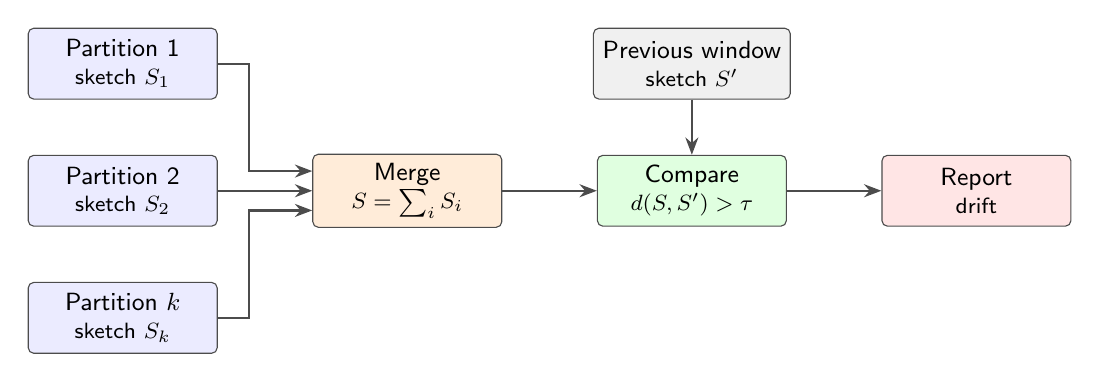
\begin{tikzpicture}[font=\sffamily\small, node distance=7mm and 12mm,
  box/.style={draw=black!70, rounded corners=2pt, minimum width=24mm, minimum height=9mm, align=center, fill=#1},
  box/.default={blue!8}, arr/.style={-{Stealth[length=2.2mm]}, thick, black!70}]
  \node[box] (p1) {Partition 1\\[-1pt]\footnotesize sketch $S_1$};
  \node[box, below=of p1] (p2) {Partition 2\\[-1pt]\footnotesize sketch $S_2$};
  \node[box, below=of p2] (p3) {Partition $k$\\[-1pt]\footnotesize sketch $S_k$};
  \node[box=orange!15, right=of p2] (merge) {Merge\\[-1pt]\footnotesize $S = \sum_i S_i$};
  \node[box=green!12, right=of merge] (cmp) {Compare\\[-1pt]\footnotesize $d(S, S') > \tau$};
  \node[box=red!10, right=of cmp] (rep) {Report\\[-1pt]\footnotesize drift};
  \node[box=gray!12, above=of cmp] (prev) {Previous window\\[-1pt]\footnotesize sketch $S'$};
  \draw[arr] (p1.east) -- ++(4mm,0) |- ([yshift=2.5mm]merge.west);
  \draw[arr] (p2) -- (merge);
  \draw[arr] (p3.east) -- ++(4mm,0) |- ([yshift=-2.5mm]merge.west);
  \draw[arr] (merge) -- (cmp);
  \draw[arr] (prev) -- (cmp);
  \draw[arr] (cmp) -- (rep);
\end{tikzpicture}
\end{document}
